\documentclass{article}
\usepackage[utf8]{inputenc}
\usepackage{algpseudocode}
\usepackage{amsmath}
\usepackage{amsthm}
\usepackage{graphicx}

\newtheorem{theorem}{Theorem}
\newtheorem*{lemma*}{Lemma}

\algnewcommand{\IIf}[1]{\State\algorithmicif\ #1\ \algorithmicthen}
\algnewcommand{\EndIIf}{\unskip\ \algorithmicend\ \algorithmicif}
\algnewcommand{\True}{\textbf{true}}
\algnewcommand{\False}{\textbf{false}}

\title{CS166 Final Project: \\ Decremental Tree Connectivity}
\author{Gawan Fiore, Nick Troccoli, Nikhil Desai}
\date{June 2018}

\begin{document}

\maketitle

\section{Introduction}
The decremental tree connectivity (DTC) problem is the problem of tracking whether two nodes in a tree remain connected after an arbitrary number of edge deletions.  Specifically, starting with a tree $T$ consisting of $n$ nodes and at most $n-1$ edges, we must support the following two operations: \\ \\
\textbf{delete(e)} $\rightarrow$ deletes the edge $e$. \\
\textbf{connected(a,b)} $\rightarrow$ returns a boolean value indicating whether nodes $a$ and $b$ are connected. \\ \\
As trees are special formations of a graph, the algorithm and accompanying data structure are special cases of the dynamic decremental connectivity approach for generalized graphs. However, the special property of trees - that two nodes have at most 1 path between them - allows for a significant speed-up. \\ \\
The ultimate goal for solving this problem on trees is to create a data structure and algorithm that allows us to make connectivity queries in constant time and deletions in amortized constant time such that over the entire lifetime of the data structure, at most $n-1$ deletions takes time $O(n)$ and thus the total runtime for fully using this data structure is $O(q + n)$, where $q$ is the number of connectivity queries made by the user. Note that this data structure only has at most $n-1$ edges to begin with, so that is the maximum number of deletions possible. \\ \\
Finally, we propose a variant of this data structure and algorithm supporting more generalized tree connectivity functionality, allowing node+edge insertions in addition to deletions while maintaining the optimal amortized constant runtime for queries, deletions, and insertions.

\section{Applications}
As mentioned in Alstrup, Secher, and Spork's paper \cite{ALSTRUP1997161}, DTC can be used as a subroutine for randomized algorithms on graph connectivity. They also demonstrate its applicability for a particular case of the UNION\_FIND problem. More generally, however, this data structure has applications to network outage detection in communication lines, water and electricity delivery, road congestion maps, among many others. Any system that can be modeled as a tree or forest graph is a possibility, in addition to those that are connected graphs, via the randomized subroutine method mentioned above. \\

\section{Naive solutions to decremental tree connectivity}
Approaching this problem from a naive perspective, we see two easy solutions: (1) optimize entirely for connectivity query time, (2) optimize entirely for deletions of edges.

\subsection{Edge deletions in time $O(1)$}
We do nothing to augment the tree, handling deletions and queries as they come: \\ \\
\textbf{delete(e)} $\rightarrow$ deletes the edge $e$. The runtime is $O(1)$ for a single deletion, or $O(n)$ over all deletions in the lifetime.  \\
\textbf{connected(a,b)} $\rightarrow$ traverses the tree from node $a$ to node $b$, and return whether or not we can reach $b$. The worst case runtime is $O(n)$ if the queries are always for nodes on opposite sides of the tree. \\ \\
That makes it very efficient to delete edges, but it's very slow to determine if nodes are connected, which is the whole point of the data structure. In total, we have a runtime of $O(q + n^2)$ for $q$ queries and at most $n-1$ deletions.  In many cases we can assume that we're going to be getting many more queries than we have nodes, so let's try the other extreme.

\subsection{Connectivity queries in time $O(1)$}
Perhaps some pre-processing and augmentation will help. Let's assign each node with a number indicating what component it's a part of.  Initially, we will assign each node a component ID of 0. Store these IDs in an array that can be constructed in time $O(n)$.
\textbf{delete(e)} $\rightarrow$ deletes the edge and assigns a new ID to all nodes in the newly created left connected component and a new ID to all nodes the newly created right connected component. The worst case runtime is $O(n)$ for a deletion, or $O(n^2 + n) = O(n^2)$ over all deletions in the lifetime.  \\
\textbf{connected(a,b)} $\rightarrow$ checks our ID-tracking array at index $a$ and index $b$. If they're equal, they must be in the same connected component, so return true; if they're different, return false. Runtime: $O(1)$ per query. \\ \\
We achieved our $O(1)$ connectivity query, but at the cost of an $O(n^2)$ total deletion time. Can we do better?

\section{A $O(n\log n)$ implementation on tree graphs}

In 1981 Even and Siloach \cite{Shiloach} derived a new method that would become a building block of the optimal online DTC algorithm we have today. Their paper focused mainly on generalized graph decremental connectivity, but, as trees and forests are a type of graph, they included a section on their fastest approach for solving the specialized tree scenario in time $O(1)$ for queries and $O(n \log n)$ for all edge deletions over the course of the entire life of the data structure. Thus any data structure's lifetime runtime is $O(q + n \log n)$, where $q$ is the number of connectivity queries made. It is constructed as follows: \\ \\
First, the easy part - connectivity queries. A table is constructed with an entry for each vertex in the initial tree. In the table, each entry at index $i$ holds the ID number of the connected component that vertex $i$ belongs to - these start at 0 and are incremented each time a new connected component is introduced. As a result, any query $connected(a,b)$ can be answered in constant time by determining if the component IDs of $a$ and $b$ match (thus indicating that they are in the same connected component). That's an optimal query time, and matches the approach of the second naive implementation, but what about deletions of edges? They achieved $O(n \log n)$ total deletion time by examining the tree as follows.  Because $T$ is a forest, the deletion of an existing edge, $e$, will break a connected component into two smaller connected components. Starting at each of the two vertices of $e$ we can scan away from $e$ in parallel until one of the two scans has explored all vertices in its connected component - this is the smaller of the two new connected components. Then the table entries for all of the vertices in the smaller component are updated to a new connected component ID, which is the previous ID incremented by 1. All entries for vertices in the other component are unchanged. The total time of this operation is $3n = O(n)$, where $n$ is the number of vertices in the smaller component: $n$ constant traversals in the scan on the smaller component, $n$ constant traversals in the scan on the larger component (with its scan cut short), and one constant table update operation on each of the $n$ vertices in the smaller component. Thus, it is a constant amount of work per vertex in the smaller component. \\ \\
This is a step in the right direction, but it still seems like it might take worst case $O(n)$ time to perform a deletion, where $n$ is the total tree size. The necessary observation is that each vertex can be in a smaller connected component after an edge deletion at most $\log n$ times. To see why this is true, let's track an arbitrary vertex $a$. The best case scenario is when $a$ is never in the smallest connected component; wonderful, we've done no work. The worst case scenario is when $a$ is in the smallest connected component every time until it is a singleton tree. If each edge deletion splits $a$'s component in half, and $a$ is always in the smaller sub-component, $a$'s component can only be halved $\log n$ times before $a$ has no edges and thus cannot be involved in further edge deletions. \\ \\
The final result is that each vertex in the tree does constant work in at most $\log n$ deletion operations, yielding a worst-case runtime of $O(n \log n)$ over the data structure's lifetime. Combined with $q$ constant queries and the preprocessing time for table construction, we have $O(q + n \log n + n) = O(q + n \log n)$. \\ \\
This approach is used directly in the top-level data structure for the optimal online DTC algorithm discussed in the next section.

\section{DTC}
We've seen above an algorithm for a tree of size $n$ that can execute the worst case number of delete operations, and an arbitrary number of queries, in $O(q + n \log n)$ time.  But we can do even better.  Stephen Alstrup, Jens Peter Secher, and Maz Spork from the University of Copenhagen proposed an even faster version with $O(q + n)$ cumulative time for these operations.  The key insight they made is that the dynamic tree connectivity problem can be broken up into multiple smaller dynamic tree connectivity problems.  For example, given a tree, we could divide the tree into several smaller "microtrees", each of which is a decremental tree connectivity problem.  We could then model the whole tree as a "macrotree" decremental tree connectivity problem between these smaller trees - considering just their "boundary" nodes, or the nodes that join them.

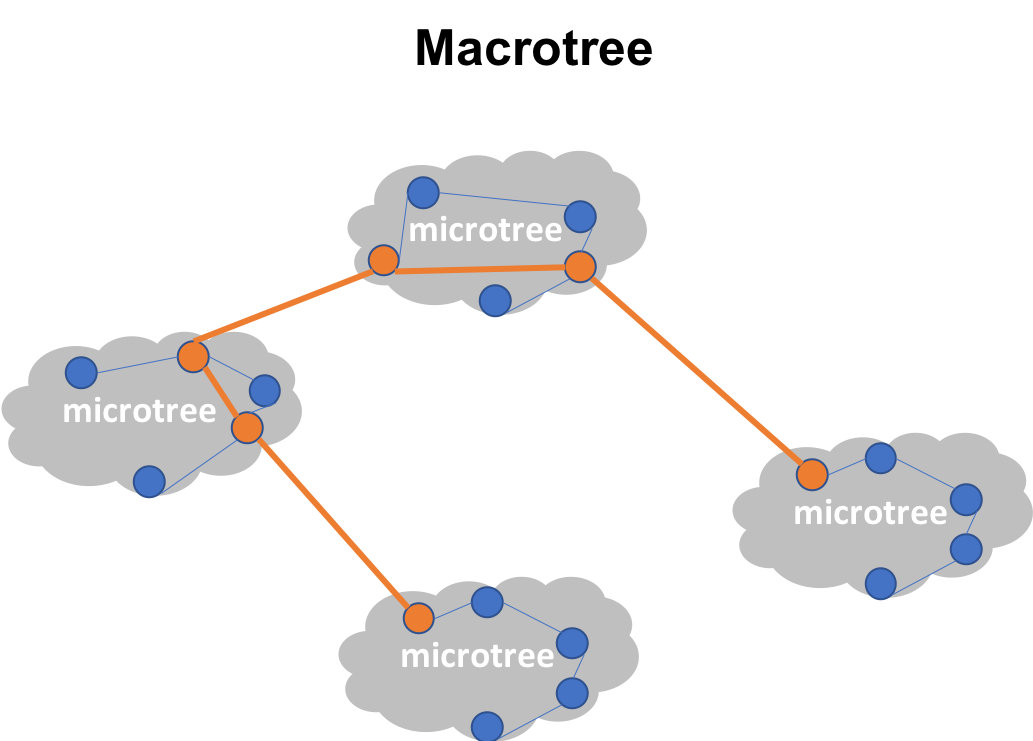
\includegraphics[scale=0.6]{DTC.png}\\

To delete an edge, we could delete it from the microtree that contains it, and potentially from the macrotree if it affects connectivity between microtrees.  To answer connectivity queries, if the connectivity query is contained entirely within a single microtree, we can just query that tree for the answer.  If the query is across multiple microtrees, we can query both the macro- and micro- trees along the path between the nodes to get our answer.  To more fully understand this approach, we'll go more in depth about what these two types of trees are, and how they work together.

\subsection{macro layer}
Our intuition has suggested that a ``two-tiered" approach, akin to that used in common RMQ structures, will allow us to speed up dynamic connectivity queries on trees. We need to answer three questions about this approach to verify that it will be optimal. First, given some partition of the tree into ``micro" and ``macro" structures, how would we combine information from these structrues to answer connectivity queries, and how would we update them after an edge deletion? Second, what would be the optimal number and size of the partitions (i.e., the microtrees) of our initial data? And third, how can we assign the nodes of a single tree to different microtrees, as well as possibly to the macrotree? We answer the first question in this section and touch on the third, which requires some more complicated mathematics for a rigorous treatment. We defer the second question to the later section on runtime.

\paragraph{Algorithms for the overall structure:}
As it turns out, answering connectivity queries in the two-tiered structure is straightforward when we choose our low-level structures to be tree-shaped, as long as we intelligently pick representatives of each micro structure to sit in the macro structure. In particular, imagine that we create micro-structures representing contiguous subsets of the tree. For each micro-structure, we pick its ``boundary" nodes, those that are connected to at least one node outside their micro-structure, to also inhabit the macro-structure. We add all edges between these boundary nodes that are found in the original tree as edges of the macro-structure; in addition, we draw edges between all boundary nodes in the macro tree that are associated with the same micro tree. Observe that any edge in the graph either connects two nodes in the same micro-structure - in which case the edge is faithfully represented there - or connects two nodes in different micro-structures - in which case they are both boundary nodes, and the edge is faithfully represented in the macro-structure. Thus, every edge in the tree, and its corresponding connectivity information, is captured somewhere in our structure.

Once this is done, we will have a large group of tree-shaped micro-structures representing contiguous subsets of the original tree, and a macro-structure (not necessarily tree-shaped) that encodes the connectivity between representatives of these micro-structures. The question still remains - how can we use this structure to check if two arbitrary nodes are connected? It turns out the algorithm to check this is straightforward, because our partitioning into macro and micro structures pays off here. In particular, for two nodes $v$ and $w$ in the tree, either they are in the same micro-structure or they are not. If they are, we can just query that micro-structure for whether or not they are connected. If they are not, we can look at all of the boundary nodes of their trees, see if any of the boundary nodes are connected, and then check if those boundary nodes are connected back to our original $v$ and $w.$ More formally, let's assume we  have access to primitives $tree(v)$ and $boundaries(v)$ that find $v$'s microtree and its boundary nodes, respectively. We also assume the (for now undefined) procedures $\textsc{Macrocon}(v,w)$ and $\textsc{Microcon}(v,w,T)$, which check whether the nodes $v$ and $w$ are connected in the macro structure and the micro structure T, respectively. Then the following algorithm will return \textbf{true} if and only if there is a path between $v$ and $w.$

\begin{algorithmic}
    \Procedure{Con}{$v,w$}
            \For{$a$ in $boundaries(v)$}
                \For{$b$ in $boundaries(w)$}
                \If{\Call{Helper}{$v,a,b,w$}} \Return{\True}\EndIf
                \EndFor
    		\EndFor
    		\State \Return{\False}
    \EndProcedure
    
    
    \Procedure{Helper}{$v,a,b,w$}
            \State $T_1 \gets tree(v)$
            \State $T_2 \gets tree(w)$
            \State \Return{\Call{Microcon}{$v,a,T_1$} and 
                \Call{Macrocon}{$a,b$} and
                \Call{Microcon}{$b,w,T_2$}}
    \EndProcedure
\end{algorithmic}

The procedure for deleting an edge from the tree is also relatively straightforward. If the edge to be deleted exists between two nodes of the macro-structure, we can delete it and be done. If it's within a micro-structure, we need to delete it from there and also update the macro-structure to be aware of this possible break in connectivity. This is accomplished through the following algorithm, which again assumes the presence of the primitives $tree$ and $boundaries$ along with the routines $\textsc{Macrodelete-Edge}(a,b)$ and $\textsc{Microdelete-Edge}(v,w,T),$ which have the expected behavior.

\begin{algorithmic}
    \Procedure{Delete-Edge}{$v,w$}
            \State $T_1\gets tree(v)$
            \State $T_2\gets tree(w)$
            \If{$T_1 = T_2$}
                \For{pairs $(a,b)$ in $boundaries(v)$}
                    \If{not \Call{Microcon}{$a,b$}}
                        \State \Call{Macrodelete-Edge}{$a,b$}
                    \EndIf
                \EndFor
                \State \Call{Microdelete-Edge}{$v,w,T_1$}
            \Else
                \State \Call{Macrodelete-Edge}{$v,w$}
            \EndIf
    \EndProcedure
\end{algorithmic}

The two algorithms together seem easy enough to understand - essentially, deletions within micro-level structures get propagated up to the macro-level structure, and connectivity insights from the macro-level structure can be combined with the micro-level structures' insights to solve connectivity queries. However, we can't be sure yet if this breakdown is in any way efficient; indeed, both of our algorithms require expensive iterations over all pairs of microtree ``boundary" nodes, which in the worst case might very well be all the nodes in the microtree! (Put another way, our algorithm above would be no help if we made every node form its own micro-structure, forcing our macro tree to be formed on all $n$ nodes.)

Fortunately, there is a powerful theorem on tree graphs that means not only that this worst-case scenario won't happen, but that in all cases we can break the tree down into an essentially optimal set of micro-structures - and thus gain some pretty dramatic speedups. We'll cover the theorem in the ``Runtime" section, below, but a restricted statement of the theorem will be helpful for the next section. We state it here as a lemma.

\begin{lemma*}[Frederickson]
    For any binary tree, there exists a partition of this tree into $O(n/\log n)$ contiguous microtrees, each with at most $\log n$ nodes and at most 2 boundary nodes.
\end{lemma*}

As a consequence, we assume for the presentation of algorithms in the next section that all microtrees contain no more than $\log n$ nodes. As in the analogous Fischer-Heun structure for RMQ, the constrained size of the micro-level structures we have just proposed will be the main generator of the speedup in this algorithm. However, because of the lemma above, we can also say that the macro-structure we have proposed will have a binary tree structure - since every boundary node will be connected to at most one other boundary node from its tree, and at most two other nodes outside of its tree. Thus, the algorithms we actually use for the macro graph - our implementations of $\textsc{Macrocon}(v,w)$ and \textsc{Macrodelete-edge}($v,w$) - will be exactly the $connected(a,b)$ and $delete(e)$ algorithms proposed by Even and Shiloach in their $O(n\log n)$ implementation for DTC. As we'll show in the ``Runtime" section, this will be enough for us to gain the additional efficiency we need.

\subsection{micro layer}
The critical assumption needed about microtrees is that they can be created in linear time based on the number of nodes, and from then on support constant time edge deletions and connectivity queries.  How is this possible?  It turns out that if we limit the size of the microtrees to $\log n$ edges, we can take advantage of some clever bit-level techniques.

First, how do you build a microtree structure?  There are two items that need to be created to initialize the structure - a bit array for its edges, and \textit{rootpaths} for its nodes (we also store the original tree, and the boundary nodes for this microtree, as well as a way to map to this microtree from each node/edge in the microtree in O(1) time). The bit array keeps track of $currentEdges$, that stores which edges are in the microtree.  In other words, the \textit{i}th bit is 1 if edge \textit{i} (the edges are numbered consecutively) is in the tree, and 0 otherwise.  Because there are at most $\log n$ nodes in a microtree, we need at most $\log n$ bits.  This fact will come in handy later. This structure also precomputes something called a \textit{rootpath} for each node in the tree, other than one node that we specify as the \textit{root node}.  The root node can be any arbitrary node in the tree that we pick as the root.  For each non-root node $v$, its \textit{rootpath}, \texttt{rootpath(v)}, is the set of edges from $v$ to $r$.  We assume that the starting tree structure that we initialized with was a tree - thus, every node was reachable from the root that we chose.  Note that, like the edge bit array, we can represent rootpaths as bit arrays, too.  We can calculate all rootpaths in linear time based on the number of nodes; to do this, we can execute the following algorithm (where we assume that we can index edges and nodes by consecutive numbers):\\

\begin{algorithmic}
    \Procedure{RootPathPreprocessing}{$root$}
            \State $\Call{Helper}{root, 0}$
    \EndProcedure\\
    \Procedure{Helper}{$v$, $bitarray$}
    		\State $rootPaths[v] \gets bitArray$
    		\For{$edge$ in $v.edges$}
    		    \State $newBitArray.one(edge)$ \Comment{Mark this edge as visited in the bit array}
    		    \State $\Call{Helper}{edge.end, newBitArray}$
    		\EndFor\label{edgesLoop}
    \EndProcedure
\end{algorithmic}

This procedure visits each node exactly once, and at each node does $O(1)$ work, for a total runtime of $O(n)$, where $n$ is the number of nodes in the microtree.

Second, we'll see how we can utilize this microtree structure to delete edges and answer connected(A, B) in $O(1)$ time.  The general idea is that we'll use the rootpaths to figure out how to get from node A to node B in the \textit{initial tree}, and $currentEdges$ to figure out whether that path is still in tact after arbitrary deletions.  To delete an edge, we just set its corresponding bit in $currentEdges$ to 0, indicating that it's no longer valid to use to connect nodes.  To answer whether two arbitrary nodes A and B are connected, we first calculate a path from A to B.  A first attempt could be the path A-root-B, which would be the combination of the rootpaths of A and B.  But this may traverse some edges twice.  We can ignore these doubly-used edges using the XOR bit operator to get a shorter path by saying $path = rootPath(A) \oplus rootPath(B)$.

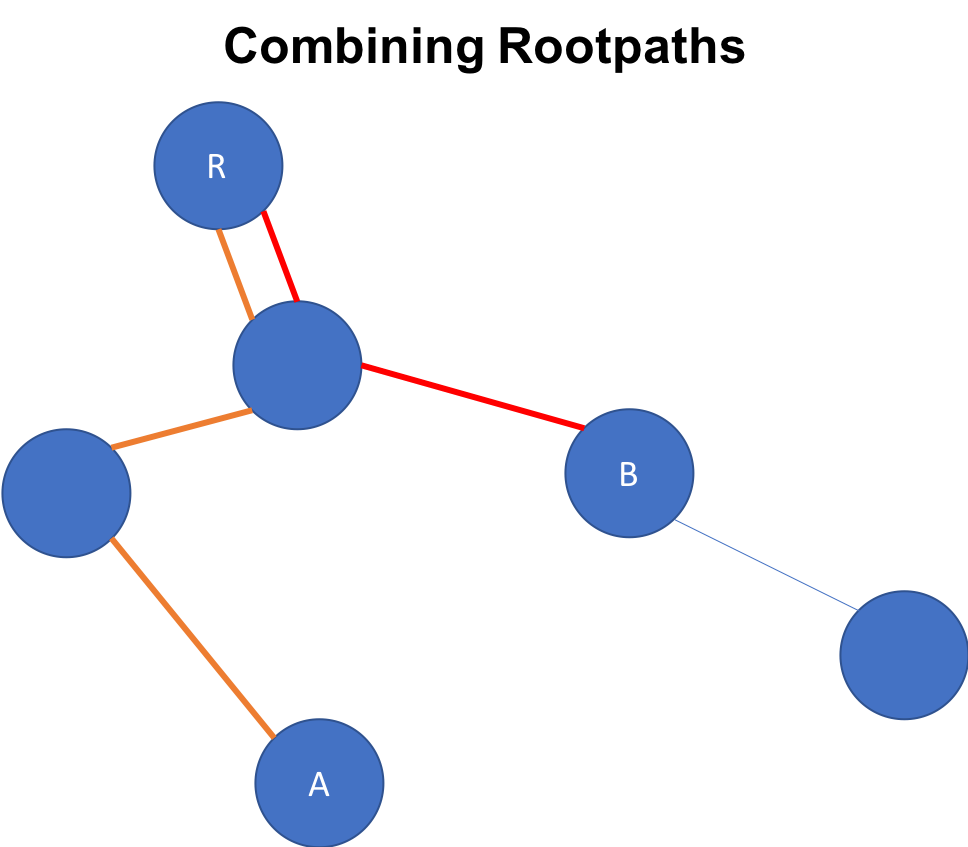
\includegraphics[scale=0.6]{rootpaths.png}\\

Then, we need to check whether all of these edges are still valid - in other words, whether they are in $currentEdges$.  The idea is that if we see any invalid edges in the inverse of $currentEdges$ that are in the path, then the path is invalid.  We can do this with the AND bit operator as follows: $isInvalid = path \& \neg currentEdges$.  If this expression evaluates to 0, then there were no edges that are invalid and in this path.  Otherwise, there are invalid edges in this path, and the path cannot be traversed.  Thus, we can implement \textsc{Microcon}$(A, B)$ as follows:

\begin{algorithmic}
    \Procedure{Microcon}{$a, b$}
        \State $\Return (rootpath(a) \oplus rootpath(b)) \& \neg currentEdges == 0$
    \EndProcedure
\end{algorithmic}

We can see that edge deletion is $O(1)$, as it just requires a single bit flip.  How is $connected$ O(1) as well?  From earlier, we know that $currentEdges$ and any rootpath can fit in at most $log n$ bits.  In this problem, we are assuming that we have at least $log n$ bits in a single machine word.  Why?  Because we need at least $log n$ bits to store $n$, which is the size of the entire tree, and in the \textit{transdichotomous machine model}, we assume that the problem size can fit into a machine word.  Thus, $currentEdges$ and each rootpath can fit into a single machine word.  For this reason, the above bit operations are constant time, as they require only 1 machine word bit operation for the XOR, 1 machine word bit operation for the negation, and a final machine word bit operation for the AND.

\subsection{runtime analysis}
In this section, we will analyze the runtime of the algorithm presented above.

\paragraph{Optimal dissection of trees:}
The key speedup of the decremental tree connectivity algorithm comes from the following theorem of Frederickson \cite{Frederickson}, which we will state with informal proof:

\begin{theorem}[Frederickson]
    For any tree with maximum degree at most 3, and for any $w,$ there exists a partition of this tree into $O(n/w)$ contiguous microtrees, each with at most $w$ nodes and at most 2 boundary nodes. Furthermore, there exists an algorithm to do this partitioning in linear time.
\end{theorem}

The (informal) proof of this comes via a greedy algorithm \cite{BilleSlides}. We can treat any tree with maximum degree 3 as a binary tree with some root, and can traverse the tree breadth-first downwards. For each node $c$ we encounter, we check its number of children (this can be done in constant time with sufficient preprocessing). If it has fewer than $w$ children, we can turn its subtree into a single microtree with $c$ as the boundary node; otherwise, we descend as far as possible in the subtree of $c$ to find a descendant node $z$, which will be the ``other end" of our microtree. We choose $z$ such that there are fewer than $w$ nodes connected to the subtree spine between $c$ and $z,$ and form these nodes into a micro-tree with boundary nodes $c$ and $z.$ Because this is a breadth-first traversal, we will visit each node only once, every node will be assigned a micro-tree, and the greediness of the algorithm will ensure every micro-tree is as large as possible within the constraints, proving the theorem.

This theorem, which was proven by Frederickson in two papers about minimum spanning trees, allows all the pieces of the algorithm presented above to click into place. With a choice of $w=\log n,$ we generate a linear-preprocessing, constant-query, and logarithmic-update data structure for the decremental tree connectivity problem. To see why this holds, we analyze the runtime of the structure in three parts: the macro runtime, the micro runtime, and the combined runtime.

\paragraph{Macro structure:}
Choosing $w=\log n$ and applying Frederickson's theorem generates  a macro-structure on $|V| = O(n/\log n)$ nodes. 

We chose \textsc{Macrocon}($v,w$) and \textsc{Macrodelete-edge}($v,w$) to be the decremental tree connectivity algorithms proposed by Even and Shiloach. After $O(|V|)$ preprocessing, we find a $O(1)$ runtime for \textsc{Macrocon} and thus a runtime of $O(q+|V|\log|V|)$ to answer $q$ queries and delete all edges via successive calls to \textsc{Macrodelete-edge}. 

Now, observe that by our definition of $|V|,$ we obtain a total runtime of $$O(q+|V|\log|V|) = O(q+(n/\log n)\cdot \log(n/\log n)) = O(q+n\log n/\log n)=O(q+n).$$ Consequently, the total time to to answer $q$ queries and delete all edges in the macro-tree will be $O(q+n).$

\paragraph{Micro structure:}
Choosing $w=\log n$ and applying Frederickson's theorem generates $O(n/\log n)$ micro-structures on at most $\log n$ nodes each.

Using the bit structure developed in the previous section, we can see that \textsc{Microcon} is implemented through a single XOR and a single AND operation on machine words, and therefore runs in constant time. In addition, \textsc{Microedge-delete} is implemented as the flip of a single bit in the node's \texttt{rootpath} bit vector, taking up a single machine word; it is is also thus $O(1)$ for a single deletion.

\paragraph{Combined runtime:}
By choosing $w=\log n$ and applying Frederickson's theorem above, we have shown that we obtain a runtime of $O(n+q)$ for answering $q$ queries and deleting all edges in the macro tree, and constant-time for all operations done on any micro tree, assuming preprocessing times linear in the sizes of the trees in both cases, along with a linear time partition. This implies that our total preprocessing time is $$O(n + n/\log n + (n/\log n)\log n)=O(n).$$

Also due to Frederickson's theorem, we know that $boundaries(v)$ is a list of at most length 2; because of this, the algorithm \textsc{Con}($v,w$) presented above makes at most 4 calls to \textsc{Macrocon} and 4 calls to \textsc{Microcon} when invoked. Furthermore, any edge deletion will make at most one call to \textsc{Macrodelete-edge} and at most one call to \textsc{Microdelete-edge}.

Because deleting all edges in the tree should delete all edges in both the micro-trees and the macro-tree, the total amount of work done by making $q$ connectivity queries and deleting all edges will be at most $$O(n + (n/\log n)\log n) + 8q = O(q+n),$$  proving the worst-case optimality of our structure.

\subsection{Handling trees with max-degree greater than 3}
The data structures and algorithms presented in this section make the assumption that the tree has a binary structure, and thus that any node in the tree has a degree at most 3. Graph-theoretic trees do not have this property, merely requiring that the graph has a single connected component and has no cycles. However, it is easy to convert an arbitrary tree on $n$ nodes to a binary tree on at most $2n$ nodes in linear time, via the following approach. For each node $v$ bordering nodes $w_1,\ldots, w_d$ with $d>3,$ replace $v$ with a path $v_1,\ldots,v_d$, delete the original edges $(v,w_i),$ and add the edges $(v_i,w_i).$ Then we can easily observe that the connectivity properties of this graph are identical to those of the original graph, with connectivity queries involving $v$ simulated by queries involving instead an arbitrarily chosen $v_i.$ Similarly, deletions of the edge $(v,w_i)$ can be simulated by deletions of the edge $(v_i,w_i).$

This approach replaces each node with degree $d>3$ by $d$ nodes of degree 3. Because the sum of all degrees in a tree is exactly $2|E|,$ which for a tree is $O(|V|),$ replacing every node with degree $d$ by $d$ replacement nodes of degree 3 will add $O(|V|)$ extra nodes to the graph. This does not alter the asymptotic properties of the graph size, and consequently the runtime analysis for binary trees remains valid on arbitrary trees under this transformation.

\section{Towards Fully Dynamic Tree Connectivity}
While optimal online DTC is a very fast data structure, it is somewhat limited in its capabilities, and thus applicability for solving a wide variety of problems. Allowing both insertion and deletion of edges would provide sufficient flexibility to model continuously changing tree networks such as telephone and internet communication channels. Specifically, the ultimate goal is optimal online fully dynamic tree connectivity: being able to add edges in constant time while maintaining the constant time query and deletion operations. \\ \\
The difficulty of constructing such a data structure stems from the fact that the partitioning of the micro trees is what allows for constant time edge deletions. Once you begin to add edges, it is possible that new edges distort root paths of the micro tree or cross micro trees in a manner that requires restructuring in order to not break the constant query and deletion times. It's complex and needs clarification. \\ \\
As such, we've identified three possible types of edge insertion: \\
(1) Adding a node and edge that connects it to the tree. \\
(2) Reinserting a previously deleted edge. \\
(3) Inserting an edge that previously did not exist. \\ \\
In the following subsections we propose a new data structure that successfully allows for amortized constant time edge insertions of type (1), above, while maintaining constant time queries and deletions. We also detail what next steps appear promising for developing a fully dynamic tree connectivity structure that supports \textit{any} type of edge insertion in amortized constant time. It is a problem that we are actively researching.

\subsection{Initialization}
Upon construction of the data structure we build $2$ times as much space into all structures than is necessary for the initial tree. This includes the macro tree, the macro-level component look-up table, each micro tree, and all bit vectors used by the micro trees. The initialization time for the DTC data structure was $O(n)$. We maintain this runtime bound because doubling our structures in size means our initialization time is $O(2n) = O(n)$.

\subsection{Insertion}
To insert, both our micro and macro trees need to support insertion, assuming that they are double the needed initial size.  Below, we describe modified versions of both structures that permit insertion in $O(1)$ time.
\subsubsection{Micro Trees}
The updated micro tree structure would have a $currentEdges$ bit array of size $2\log n$, with only $\log n$ bits initially used (unused bits are 0).  It would also store its original tree structure (nodes and edges) that it represents.  Finally, it would store an original copy of its $currentEdges$, which will be needed later.  When adding a new node $w$ and corresponding edge $e_w$ connecting to some existing node $v$, we would number that edge consecutively to give it a unique number, and flip that bit in $currentEdges$ to 1.  We would add it to the tree structure this microtree represents, and add to our mapping from nodes/edges to microtrees so we can look up in O(1) time what microtree a node/edge is in.  The next step is to calculate $rootpath(w)$.  Since $w$ connects to $v$ via $e_w$, $rootpath(w)$ is the same as $rootpath(v)$ but with the bit for $e_w$ set to 1.  In other words,
\begin{equation}
    rootpath(w) = rootpath(v) | (1 << index_{ew})
\end{equation}
The remaining operations are identical to the original micro tree - to find whether two nodes A and B are connected, we compare their rootpaths with the currentEdges to see if they are connected.

Now we must handle what happens if a microtree fills up its extra space.  When this happens, we need to split the micro tree into 2 smaller microtrees.  We can do this by using the graph splitting algorithm mentioned earlier in the paper to split the \textit{original} tree into 2 subtrees of size at most n/2, where n is the original microtree size.  Then, we must make a microtree structure for each of these original subtrees (that is double the size needed to support future growth) - we can do this using the same microtree initialization process, which is linear in the number of nodes.  We must also "carry over" any edge deletions to these new microtrees - to do this, looking at the microtree structure we are splitting, we can compare $originalCurrentEdges$ and $currentEdges$ and set those edge bits to 0 in the new microtree structures to indicate that those edges were deleted.  While making new microtrees, we may also introduce at most 2 additional boundary nodes between the new microtrees.  These nodes should be inserted into the macrotree, the process for which is discussed in the next section.  We assert that this whole  algorithm takes linear time in the number of nodes in the microtree being splitted, since the splitting algorithm is linear time, the microtree initializations are linear time, and the edge deletion transfers are linear time.

\subsubsection{Macro Trees}
The updated macro tree structure would be the same as before - it would have a table matching vertexes to their connected component number, and the original graph of nodes representing the boundary nodes between microtrees.  When adding a new node $w$ and corresponding edge $e_w$ connecting to some existing node $v$, we would assign $w$'s connected component number in our table to be the same as that of $v$, and update the tree structure represented by the macrotree.  Note that when we are inserting into the macrotree from a microtree, as mentioned in the previous section about splitting microtrees, we would be adding additional boundary nodes because of the split.  Thus, we would be adding new boundary nodes at the location of existing boundary nodes.  Therefore, we can access the existing boundary nodes in O(1) time (because we have them from the original microtree) and use that as the insertion point for the new boundary nodes.

Now we must handle what happens if a macrotree fills up its extra space.  When this happens, we initiate a full DTC rebuild - in other words, we rebuild a brand new DTC structure completely from scratch, of double the size we need, with a new macrotree and microtrees, in O(n) time, where n is the size of the tree.

\subsection{Runtime Analysis}
In order to maintain constant amortized runtimes for all of our operations we rely on the general principle that if reconstruction of a structure takes linear time, and an extra linear amount of space is included by the construction algorithm that can be used in constant time, then the construction cost of growing the structure can be amortized away by the linear number of constant time operations that must happen before a resizing is necessary. \\ \\
As mentioned in the previous section, there are two structures that can be resized in order to accommodate an increased number of edges: the microtree and the macrotree. When $O(n)$ new nodes+edges are added to the tree, we must perform a complete rebuild, which takes $O(n)$ time.  How long does it take to insert these $O(n)$ new nodes and edges?  If a microtree has space for the insertion, it takes $O(1)$ time, as mentioned earlier.  If it doeesn't have space, it takes $O(\log n)$ time to split the microtrees and insert into the macrotree.  These splits happen every $O(\log n)$ insertions.  Therefore, the total amortized runtime cost for inserting $O(n)$ new nodes and edges without rebuilding the entire structure is $O(n)$, since insertions take amortized $O(1)$.  Thus, including rebuilding the entire structure we have an overall amortized cost of $O(1)$ per insertion, since we do an $O(n)$ rebuild every $O(n)$ insertions, and each insertion takes amortized $O(1)$ time.

\subsection{Applications}
This new data structure has all of the applications of the optimal online DTC, but allows flexibility for edge to go offline and come back on. This means more effective modeling of network outages and real-life connectivity in trees, forests, and graphs.

\subsection{Next Steps}
This data structure represents a significant step toward a fully dynamic solution, but edge insertion types (2) and (3) are still pending. The following addresses our current progress toward support of these cases.

\subsubsection{Case 2: Reinsertion of deleted edges}
If the edge is simply deleted and reinserted right the solution is simple: do not modify the \textit{current\_edges} bit vector, but reset the consistent node's rootpath to be it's new parent's rootpath plus its parent edge that was reinserted. If the edge is deleted and reinserted at an unknown later time, we lose the edge information. Creating a new edge when we reinsert also isn't viable because we will eventually run out of space in the textit{current\_edges} bit vector if we do this too often. The general solution for this is as follows. \\ \\
First, we utilize the concept of node-edge pairs. Each node stores the ID of its parent edge (according to the ordering of the rootpath) that it had at time-of-creation. This overcomes the issue of running out of space in \textit{current\_edges} because we can actually re-use deleted edges.
Then, we have to follow two simple deletion and insertion rules to ensure that the rootpath is properly updated: \\ \\
(1) Anytime a node's parent edge is removed, set its rootpath bit vector $R_c = R_c$ $\&$ $R_p \oplus R_p$, where $R_p$ is the parent node's rootpath bit vector. This removes all information of the parent's path, but preserves information about the child's deleted parent edge. \\
(2) Anytime a node $c$ has its parent edge added back in, attaching it to another node $n$, set $R_c = R_c \oplus R_n$, effectively adding the new parent's rootpath information to the child's rootpath. \\ \\
What makes this case difficult to handle is micro tree splits, and we have yet to discover a consistent and fast method for maintaining this augmentation across such a split. However, this is perhaps an easier problem to solve than the ones in Case 3, below.

\subsubsection{Case 3: Arbitrary edge insertion}
We have made some progress on this case, but significant roadblocks still remain. The key concept preventing progress is that micro tree root paths assume a directionality that breaks down if edges can be inserted arbitrarily. \\ \\
We have made some progress on this case, but significant roadblocks still remain. The key concept preventing progress is that micro tree rootpaths assume a directionality that breaks down if edges can be inserted arbitrarily. \\ \\
For edge insertions that maintain the assumed directionality of the rootpaths, we have a constant time method for inserting new edges.  We utilize the same parent edge-storing method mentioned in the previous subsection. In order to prevent cycles, we must also perform a connectivity query on the two nodes at either end of the candidate edge. If they are already connected the insertion becomes a noop. This can be done in constant time. If all of this is in place, following the two rootpath alteration rules from the previous subsection allows us to do constant time edge rewiring. \\ \\
However, if a vertical directionality is not maintained, problems arise. Imagine a root's child severed from the root with a deletion and subsequently the child's grandchild is connected to the root with a new edge. This either flips the directionality of the child's tree or of the root's tree. Thus, it would appear that potentially log(n) time is necessary to fix-up the rootpaths for one of the two trees, but perhaps there is a clever series of bit-wise operations or a secondary augmentation that allows for this 'bi-directionality'. \\ \\
The general issues facing edge insertion are micro tree directionality inversions and handling cross-microtree edges that appear to require boundary node reshuffling. If these issues can be resolved, a path toward fully dynamic tree connectivity seems plausible.

\bibliography{main}
\bibliographystyle{ieeetr}
\end{document}
